\documentclass[10pt,a4paper]{article}
\usepackage[utf8]{inputenc}
\usepackage[english]{babel}
\usepackage[T1]{fontenc}
\usepackage{amsmath}
\usepackage{amsfonts}
\usepackage{amssymb}
\usepackage{subcaption}
\usepackage{makeidx}
\usepackage{graphicx}
\usepackage{fourier}
\usepackage{listings}
\usepackage{color}
\usepackage{hyperref}
\usepackage[left=2cm,right=2cm,top=2cm,bottom=2cm]{geometry}
\author{Tommy Müller, Marcus Dittrich, Vincent Noculak}
\title{Quadropolmassenspektroskopie}

\lstset{language=C++,
	keywordstyle=\bfseries\color{blue},
	commentstyle=\itshape\color{red},
	stringstyle=\color{green},
	identifierstyle=\bfseries,
	frame=single}
\begin{document}

Des Weiteren haben wir im Quadropolmassenfilter Luft untersucht. Dafür haben wir in der Kammer einen konstanten Druck von $1.2 * 10^{-6}$ mbar erzeugt und die Messung bei einer Scangeschwindigkeit von 10 $\frac{s}{u/e}$ durchgeführt. In Figure $\ref{f1}$ sieht man den aufgenommenen Datensatz und in Figure $\ref{f2}$ die Zuordnung der Peaks zu den Bestandteilen der Luft. Sauerstoff (20.95$\%$) und Stickstoff (78.08$\%$)  machen mehr als 99$\%$ der Atmosphäre aus und sind deswegen auch die beherrschenden Peaks der aufgenommenen Messung. Die Hauptpeaks befinden sich bei 28.31 u/e (Stickstoff) und 32.35 u/e (Sauerstoff) wobei es sich in beiden Fällen um einfach ionisierte Moleküle handelt. Außerdem gibt es zu beiden Bestandteilen der Luft noch einen zweiten Peak bei ca (m/q)/2, was für zweifach ionisierten Sauer- und Stickstoff spricht. Des Weiteren haben wir einen Peak für Wasser aufgenommen, welches sich vermutlich an den Wänden der Kammer abgesetzt hatte. Interessant ist außerdem das Artefakt des Datensatzes bei kleinem m/q Verhältnis. Grund dafür ist die endliche Länge des Quadropolmassenfilters und die geringen angelegten Spannungen, welche notwendig sind um kleine Massen aufnehmen zu können. Dadurch besteht allerdings die Wahrscheinlichkeit, dass unerwünschte Massen nicht mit den Stäben kollidieren und dadurch detektiert werden. Um die aufgenommenen Peaks sinnvoll zu normieren haben wir festgelegt, dass die Summe aller Partialdrücke dem Druck in der Kammer entspricht. Die ermittelten Werte haben wir in Table $\ref{as}$ dargestellt. Die dazugehörigen Fehler haben wir für m/q über die Halbwertbreite und für die Patialdrücke aus der auftretenden Druckschwankung (um 0.1 * $10^{-5}$mbar) während der Messung bestimmt. 

\begin{table}[k]
	\centering
	\caption{Bestandteile der Luft}
	\label{as}
	\begin{tabular}{|l|l|l|}
		\hline
		m/q {[}u/e{]} & p{[}$10^{-6}$mbar & Ionen \\ \hline
		14.19 $\pm$ 0.18       & 1.06  $\pm$ 0.1    & N2    \\ \hline
		16.14 $\pm$ 0.13       & 0.29  $\pm$ 0.1    & O2    \\ \hline
		18.16 $\pm$ 0.15       & 0.22  $\pm$ 0.1    & H2O   \\ \hline
		28.31 $\pm$ 0.23       & 9.32  $\pm$ 0.1    & N2    \\ \hline
		32.35 $\pm$ 0.21       & 1.09  $\pm$ 0.1    & O2    \\ \hline
	\end{tabular}
\end{table}

\begin{figure}[h]
	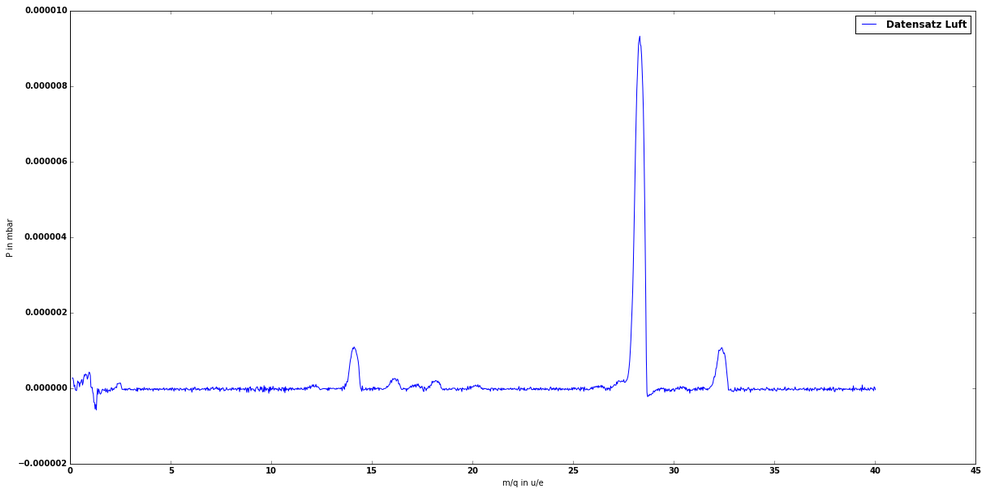
\includegraphics[scale = 0.5]{sauerroh.png}
	\centering
	\caption{Rohdaten Sauerstoff}
	\label{f1}
\end{figure}

\begin{figure}[h]
	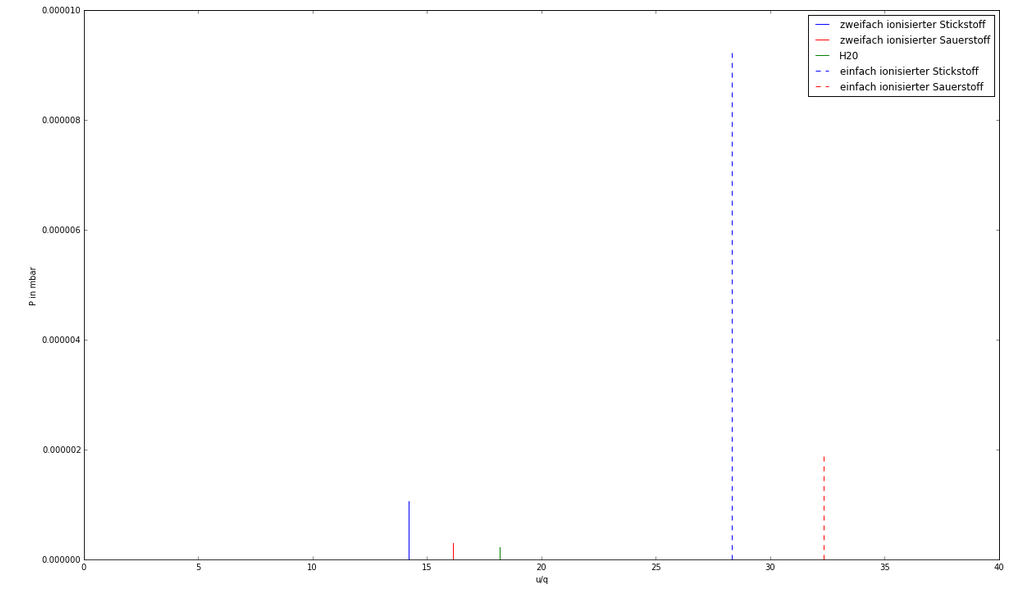
\includegraphics[scale = 0.5]{sauerstoff.png}
	\centering
	\caption{Zuordnung Peak zu Ionen}
	\label{f2}
\end{figure}
	

\section{Auflösungsvermögen}

\subsection{Massenspektren von Luft bei verschiedenen Auflösungen}

Für diesen Aufgabenteil haben wir das Massenspektrum von Luft für Auflösungen zwischen 2 und 6 aufgenommen. Dabei muss uns ein systematischer Fehler während der Messung unterlaufen sein. Im Allgemeinen erwartet man für geringere Auflösungen größere Halbwertbreiten, da ein größeres Massenintervall bei einer bestimmten Spannung den Filter passieren kann. Allerdings sind in unserem Fall die Halbwertbreiten konstant geblieben, was darauf schließen lässt, das wir die Auflösung nicht verändert haben. Ob dies an einem Fehler des Gerätes oder fehlerhafter Bedienung lag, ist für uns zum momentanen Zeitpunkt nicht nachvollziehbar. Exemplarisch haben wir in Table $\ref{t1}$  $\&$ $\ref{t2}$  die Position der Hauptpeaks und mit den dazugehörigen Halbwertbreiten dargestellt. Die Breite der Peaks haben wir mit der Software Peak-O-Mat ausgewertet. Für den Fehler vom $\Delta$m/q haben wir 0.01 u/e angenommen. Die Standardabweichung von m/q der Peaks haben wir aus dem vorherigen Aufgabenteil übernommen. Die einzelnen Messdaten der verschiedenen Auflösungen aus Figure $\ref{f3}$  $\&$ $\ref{f4}$ wurden so normiert, das die Summe aller relevanten Peaks 1 ergibt.
\begin{figure}[h]
	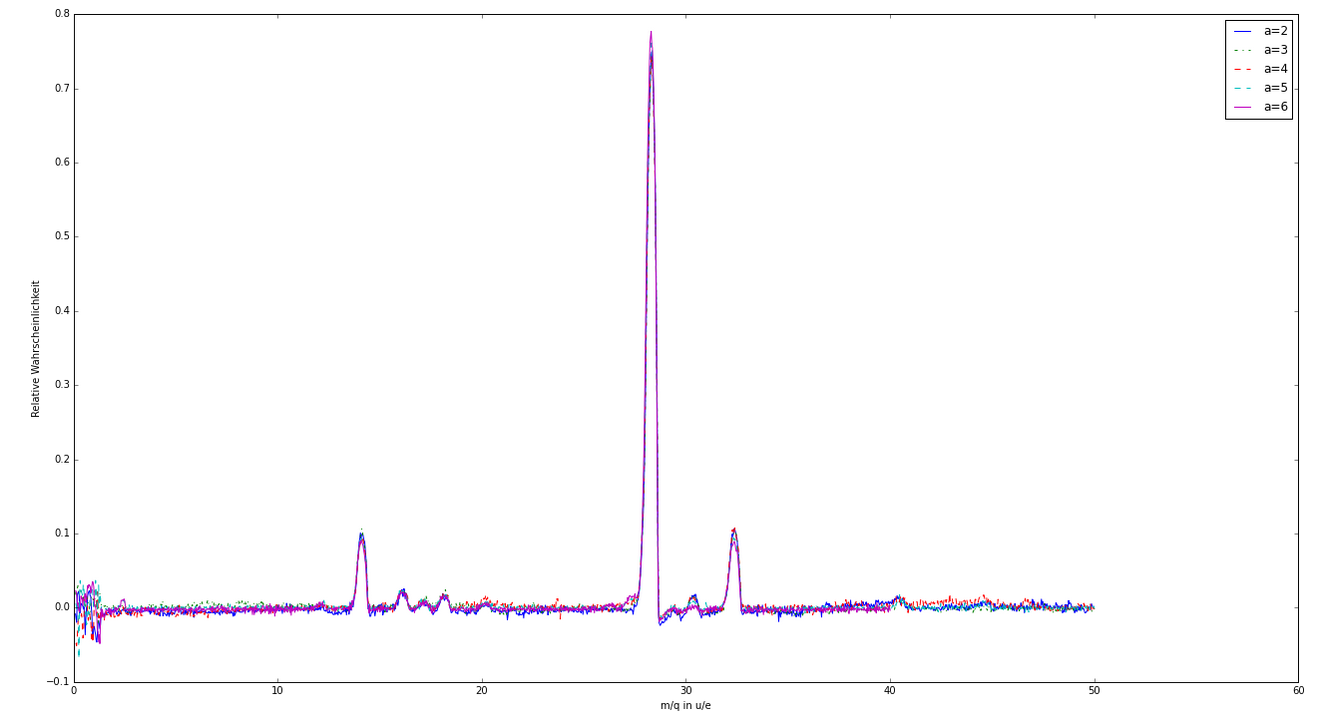
\includegraphics[scale = 0.5]{alleres.png}
	\centering
	\caption{Überlagerung der Rohdatensätze aller Auflösungen}
	\label{f3}
\end{figure}
\begin{figure}[h]
	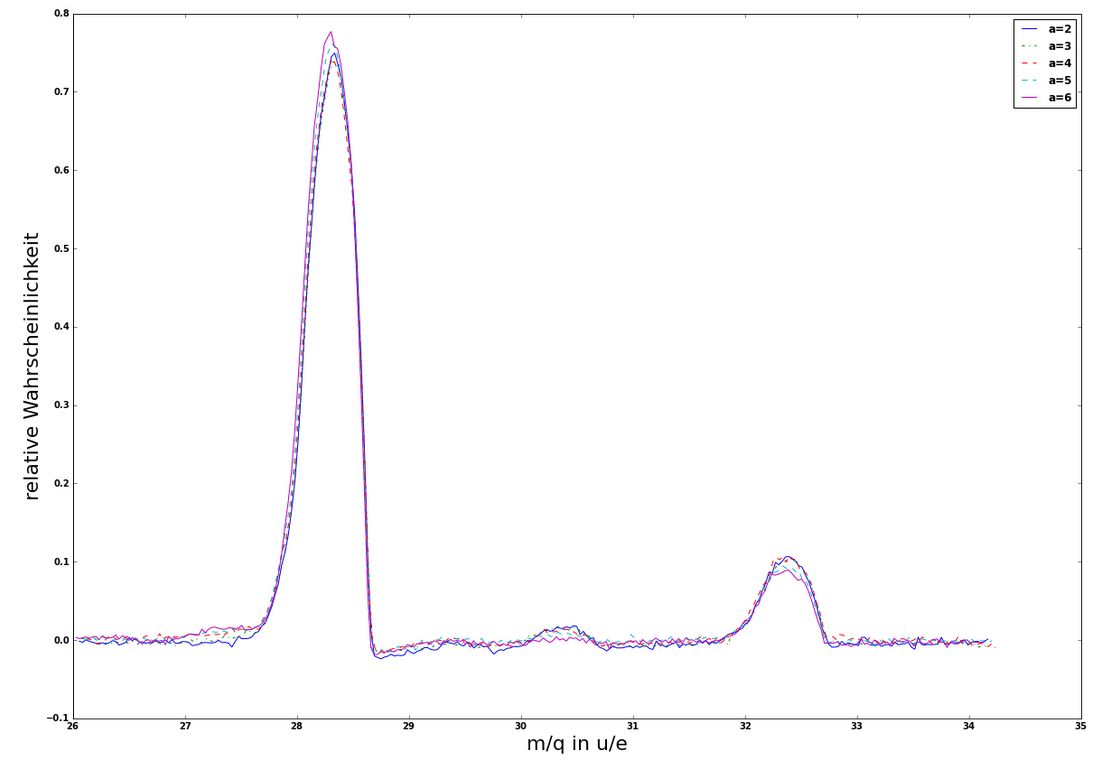
\includegraphics[scale = 0.5]{zweipeaks.png}
	\centering
	\caption{Überlagerung der Hauptpeaks}
	\label{f4}
\end{figure}
\begin{table}[k]
	\centering
	\caption{N2 Peak}
	\label{t1}
	\begin{tabular}{|l|l|l|}
		\hline
		Auflösung & m/q {[}u/e{]} & $\Delta$m/q {[}u/e{]} \\ \hline
		2         & 28.33 $\pm$ 0.23        & 0.53 $\pm$ 0.1                 \\ \hline
		3         & 28.34 $\pm$ 0.23        & 0.56 $\pm$ 0.1                 \\ \hline
		4         & 28.32 $\pm$ 0.23        & 0.53 $\pm$ 0.1                 \\ \hline
		5         & 28.32 $\pm$ 0.23        & 0.55 $\pm$ 0.1                 \\ \hline
		6         & 28.30 $\pm$ 0.23        & 0.53 $\pm$ 0.1                 \\ \hline
	\end{tabular}
\end{table}
\begin{table}[k]
	\centering
	\caption{O2 Peak}
	\label{t2}
	\begin{tabular}{|l|l|l|}
		\hline
		Auflösung & m/q {[}u/e{]} & $\Delta$m/q {[}u/e{]} \\ \hline
		2         & 32.38 $\pm$ 0.21         & 0.51 $\pm$ 0.1                 \\ \hline
		3         & 32.37 $\pm$ 0.21         & 0.52 $\pm$ 0.1                 \\ \hline
		4         & 32.39 $\pm$ 0.21         & 0.49 $\pm$ 0.1                 \\ \hline
		5         & 32.37 $\pm$ 0.21         & 0.51 $\pm$ 0.1                 \\ \hline
		6         & 32.38 $\pm$ 0.21         & 0.55 $\pm$ 0.1                 \\ \hline
	\end{tabular}
\end{table}

\begin{figure}[h]
	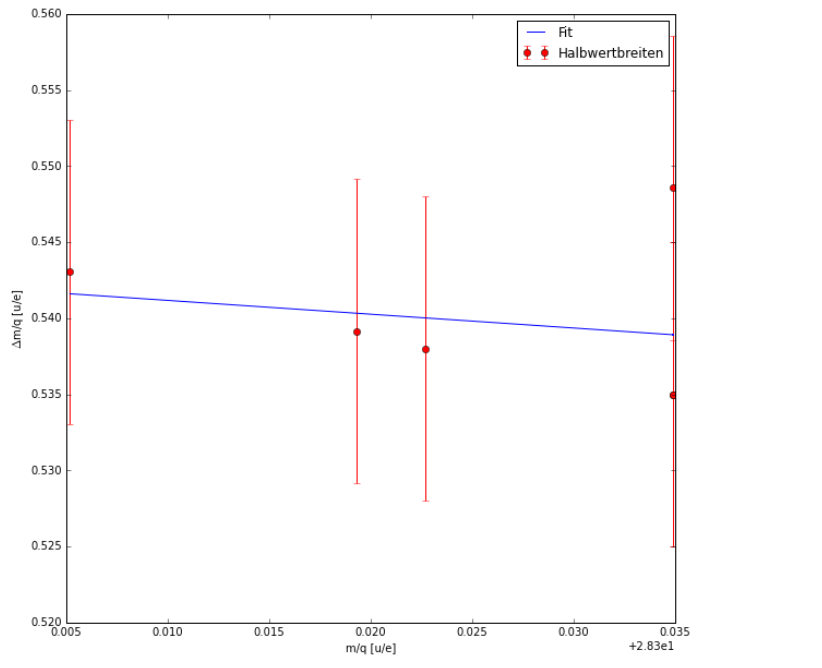
\includegraphics[scale = 0.5]{linpeak1.png}
	\centering
	\caption{Lineare Regression N2 Peak}
	\label{f5}
\end{figure}
\begin{figure}[h]
	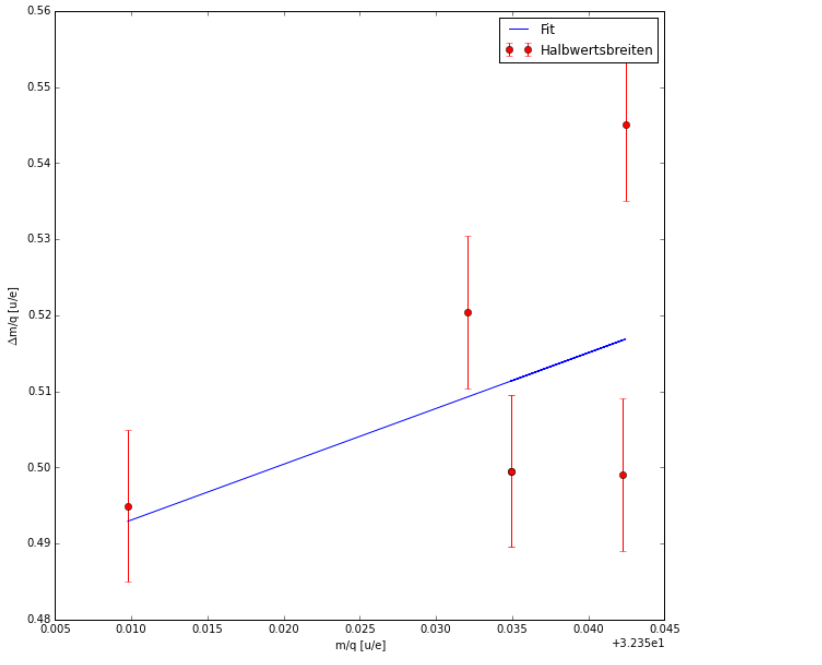
\includegraphics[scale = 0.5]{linpeak2.png}
	\centering
	\caption{Lineare Regression O2 Peak}
	\label{f6}
\end{figure}


Veranschaulichend haben wir in Python die lineare Regression auf die ermittelten Werte angewandt und dies in Figure $\ref{f5} \& \ref{f6}$ dargestellt. Wie im vorherigen Aufgabenteil beschrieben, ist im Quadropolmassenfilter m/$\Delta$m annähernd konstant. Somit müsste man zwei Fit-Geraden mit nahezu gleicher Steigung erhalten. In unserem Falle besitzen die beiden linearen Fits sogar unterschiedliche Vorzeichen, was die nicht vorhandene Aussagekraft unserer Messungen nochmals unterstreicht. 
\section{Diskussion}
Bei der Untersuchung von Luft konnten wir beweisen, das sich diese zum überwiegenden Teil aus Stickstoff und Sauerstoff zusammensetzt.
Des Weiteren konnten wir Kondenswasser in der Vakuum-Kammer nachweisen.

Im Aufgabenteil 6.b. war es uns nicht möglich den linearen Zusammenhang zwischen m/$\Delta$m nachzuweisen, da unsere experimentell ermittelten Werte nicht aussagekräftig waren. 

\end{document}